\section{Marco teórico, conceptos clave del ML}\label{sec:marco-teorico}

\begin{quote}
    `\gls{ml}: the use and development of computer systems that are able to learn and adapt without following explicit instructions, by using algorithms and statistical models to analyse and draw inferences from patterns in data'\ \cite{machinel18:online}
\end{quote}

Es decir, un sistema que es capaz de inferir patrones de unos datos y realizar predicciones sobre nuevos datos a raíz de los patrones encontrados. 


\subsection{Tipos de aprendizaje y modelos}

Hay cuatro tipos de aprendizaje en el ML:\@ supervisado, no supervisado, semi-supervisado y de refuerzo\ \cite{homl56}.
Como parte de nuestros datos están etiquetados, podemos utilizar tanto el aprendizaje supervisado como el semi-supervisado. En un sistema supervisado se requiere que todos los datos estén etiquetados con la categoría deseada, en nuestro caso la contaminación. Sin embargo, para el semi-supervisado no es necesario que todos los datos estén etiquetados, pues utilizan tanto los datos etiquetados como los que no (datos parcialmente etiquetados) para tratar de generalizar mejor\ \cite{homl56}.

No utilizaremos el no supervisado, pues consiste en un conjunto de técnicas utilizadas para agrupar automáticamente datos no etiquetados a base de similitudes sin tener supervisión previa. El objetivo es que los datos dentro de un mismo grupo sean más similares entre sí que con los otros grupos\ \cite{Clustera13:online}. Sin embargo, como tenemos una cantidad más o menos considerable de información etiquetada, no nos hace falta.

Tampoco utilizaremos el aprendizaje por refuerzo, pues no se encuentra implementado dentro de la librería que utilizamos \textit{\href{https://scikit-learn.org/stable/}{sklearn}} y tampoco está dentro de los objetivos del proyecto.


\subsection{Fases del desarrollo de un proyecto de ML}

Nuestro proyecto ha tenido las fases que nombramos a continuación:

\begin{enumerate}
    \item Obtención de datos (\textit{Sección\ \ref[Sección]{sec:obtencion}})
        \begin{enumerate}
            \item Recolección de información de los \acrshort{bil}.
        \end{enumerate}
    \item Preparación de datos (\textit{Sección\ \ref{sec:preprocesado}})
        \begin{enumerate}
            \item Selección de métodos de preprocesado
        \end{enumerate}
    \item Entrenamiento de los modelos (\textit{Sección\ \ref{sec:entrenamiento}})
        \begin{enumerate}
            \item Entrenamiento `básico' de modelos
            \item Selección y refinamiento
        \end{enumerate}
    \item Evaluación de resultados
        
    \item Monitoreo de los modelos
\end{enumerate}

Podemos generalizar los procesos de un proyecto de \gls{ml} mediante el esquema de la \textit{Figura\ \ref{fig:ml-development-cycle}}. Cabe destacar que el proceso de entrenar un modelo de \gls{ml}, como bien muestra la imagen, es un proceso cíclico en búsqueda de mejores resultados a base de probar metodologías distintas, añadir pasos, el cambio de requisitos, etc.

\begin{figure}[!htb]
    \centering
    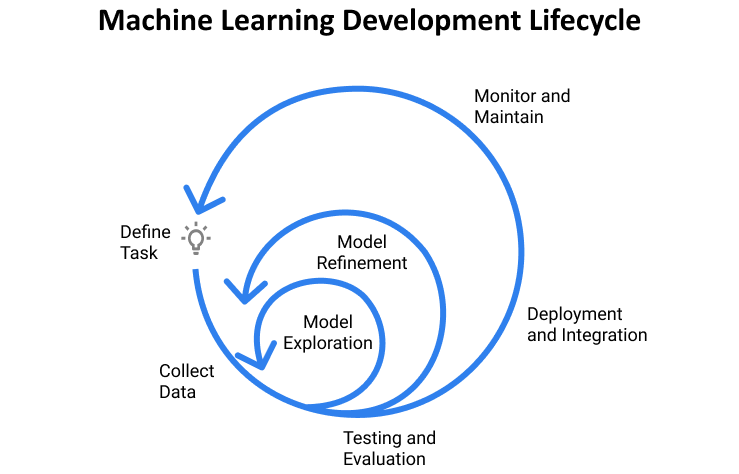
\includegraphics[width=\linewidth]{media/images/ml-development-cycle.png}
    \caption{Esquema del proceso del desarrollo de un proyecto de \gls{ml}, fuente\ \cite{Organizi22:online}}\ \label{fig:ml-development-cycle}
\end{figure}


\subsection{Métricas de evaluación de modelos}\ \label{sec:metrics}

Para el entrenamiento de modelos, su mejora y la selección de pasos del preprocesado; necesitamos algún tipo de métrica para evaluar y comparar los resultados. A continuación, explicaremos la que hemos utilizado, pero antes indagaremos un poco en su significado y sus implicaciones.

Antes de comentar la métrica que utilizaremos, explicaremos las partes de una matriz de confusión como la que podemos ver en la \textit{Figura\ \ref{fig:confusion-matrix-example}}, pues es un elemento fundamental en un modelo de clasificación. Podemos ver que tiene cuatro partes:

\begin{itemize}
    \item \textit{True Positive (tp)}, las muestras que el modelo clasifica como positivas que realmente son positivas.
    \item \textit{False Positive (fp)}, las muestras que el modelo clasifica como positivas que realmente son negativas.
    \item \textit{True Negative (tn)}, las muestras que el modelo clasifica como negativas que realmente son negativas.
    \item \textit{False Negative (fn)}, las muestras que el modelo clasifica como negativas que realmente son positivas.
\end{itemize}

Estos cuatro valores son la base del resto de métricas que comentaremos a continuación, ya que son los valores que se utilizan para calcularlas. \cite{Precisio23:online}

\begin{figure}[!ht]
    \centering
    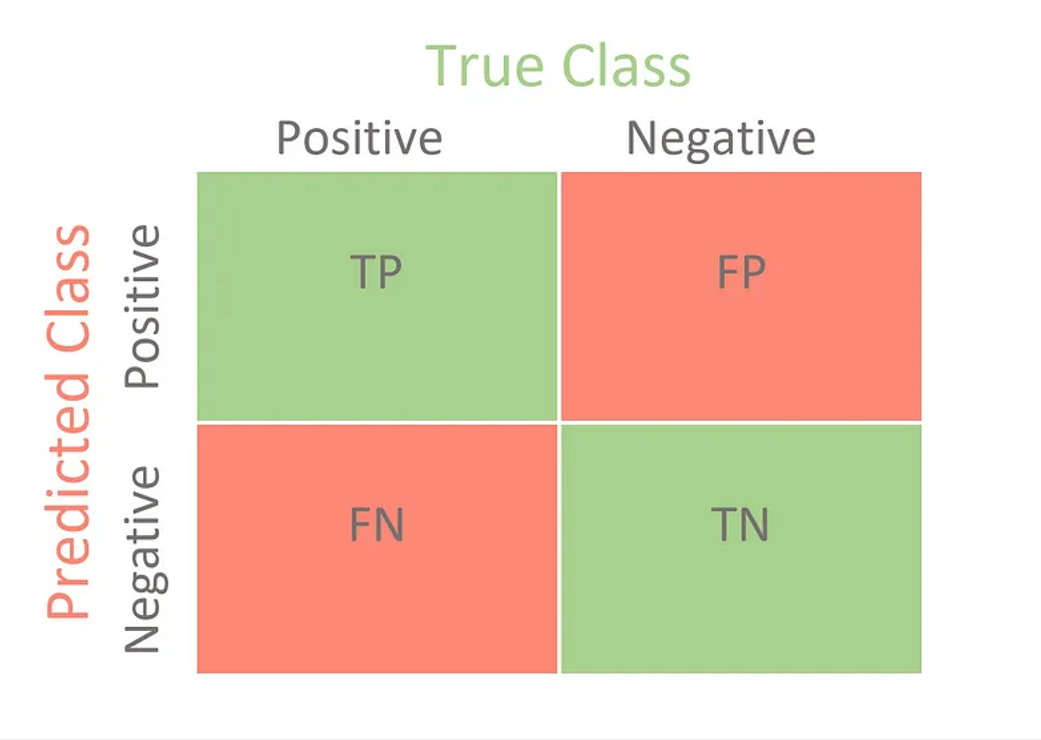
\includegraphics[width=0.7\linewidth]{media/images/confusion-matrix-example.png}
    \caption{Ejemplo de matriz de confusión, fuente\ \cite{Confusio71:online}}\ \label{fig:confusion-matrix-example}
\end{figure}
\textit{\textbf{Sensitivity}} permite saber la probabilidad de que una predicción positiva sea realmente positiva.
    \begin{equation}
        sensitivity=tp/(tp+fn)
    \end{equation}
\textit{\textbf{Specificity}} permite saber la probabilidad de que una predicción negativa sea realmente negativa.
\begin{equation}
        specificity=tn/(tn+fp)
    \end{equation}
\textit{\textbf{Recall}} indica la capacidad del modelo para encontrar todas las muestras positivas. 
    \begin{equation}
        recall=tp/(tp+fn)
    \end{equation}
\textit{\textbf{Precision}} indica la precisión de las predicciones positivas, es decir, la habilidad del clasificador para no predecir como positiva una muestra que es negativa.
    \begin{equation}
        precision=tp/(tp+fp)
    \end{equation}

Con estas métricas básicas podemos definir la que realmente utilizaremos ya que tiene en cuenta el balanceo del \gls{dataset}.

\textit{\textbf{Balanced accuracy}} es la media aritmética de \textit{Sensitivity} y \textit{Specificity}. Se utiliza principalmente cuando tratamos con datos desbalanceados\ \cite{Balanced44:online}. Su valor representa la exactitud media del modelo en las diferentes clases representadas por los datos, en nuestro caso, la clase de ``CONTAMINADO'' o ``NO CONTAMINADO''. Este valor, representa la exactitud con la que el modelo es capaz de clasificar las muestras de las diferentes clases, teniendo en cuenta la distribución de la clase mayoritaria. Es decir, si el valor de \textit{balanced accuracy} se acerca al 1, el modelo es capaz de clasificar correctamente las muestras de las diferentes clases, mientras que si se acerca a 0, el modelo no es capaz de clasificar correctamente las muestras o se aprovecha del desbalance de los datos, prediciendo mucho más la clase mayoritaria.
\begin{equation}
    balanced\_accuracy =\frac{sensitivity + specificity}{2}
\end{equation}

\subsection{Selección de modelos}

Una vez tenemos definida la métrica que utilizaremos para evaluar los modelos, necesitamos definir los modelos con los que entrenar.
Hemos seleccionado los siguientes modelos para entrenar y comparar, los cuales explicaremos brevemente, hemos intentado agruparlos por categorías.

\begin{itemize}
    \item \textbf{Árboles de decisión}: Basan sus decisiones en condiciones en estructura de árbol. Suelen ajustarse mucho a los datos, lo cual no garantiza una buena generalización de las predicciones. Suelen funcionar bien con pocos datos.
    \begin{itemize}
        \item \textit{Decision Tree} son los más básicos, dividen los datos en función de sus características. \cite{Decision70:online}
        \item \textit{Random Forest} consiste en la unión de diversos \textit{Decision Trees}, siendo la decisión final la decisión media de los mismos. \cite{RandomFo84:online}
        \item \textit{Extra Trees} de forma parecida al \textit{Random Forest}, entrena diferentes \textit{Decision Trees} sobre diferentes subconjuntos de los datos. \cite{ExtraTre48:online}
    \end{itemize}
         \item \textbf{Análisis discriminante}: Aproximan superficies de decisión en función de la clase de las muestras.
        \begin{itemize}
            \item \textit{Linear Discriminant Analysis} aproximan una superficie de decisión con un límite lineal. \cite{LinearDi2:online}
            \item \textit{Quadratic Discriminant Analysis} aproximan una superficie de decisión con un límite cuadrático. \cite{Quadrati79:online}
        \end{itemize}
    \item \textbf{Modelos basados en \textit{cercanía}}: Deciden la clase de una muestra en función de la clase de las muestras más cercanas.
        \begin{itemize}
            \item \textit{K-Neighbors} decide la clase de una muestra en función de la clase de las \textit{K} muestras más cercanas sobre las que se ha entrenado el modelo.
        \end{itemize}
    \item \textbf{Modelos basados en \textit{Gradient Boosting}}: Combinan modelos más simples, normalmente árboles de decisión, para producir un modelo más preciso y robusto.\ \cite{Gradient97:online}
    \begin{itemize}
        \item \textit{XGBoost} y \textit{LightGBM}, ambos son implementaciones de \textit{Gradient Boosting} con la mayor diferencia siendo que en \textit{XGBoost} los árboles crecen de forma profunda y en \textit{LightGBM} de forma ancha. \cite{XGBoostv70:online}  
    \end{itemize}
    \item \textbf{Modelos basados en redes neuronales}: Basados en el funcionamiento del cerebro humano, estos modelos se entrenan en función de pesos y \textit{bias}.
        \begin{itemize}
            \item \textit{Multi-Layer Perceptron classifier} red neuronal con múltiples capas de neuronas. \cite{Multilay51:online}
        \end{itemize}
    \item \textbf{Otros}:
    \begin{itemize}
        \item \textit{Stochastic Gradient Descent classifier} entrena internamente un modelo  \textit{Support Vector Machine} utilizando un método \textit{Gradient Descent} para optimizar la función de pérdida en cada iteración. \cite{SGDClass46:online}
    \end{itemize}
\end{itemize}

Exceptuando \textit{LightGBM} y \textit{XGBoost}, todos los modelos seleccionados están implementados en la librería \textit{sklearn}. Hemos considerado agregar estos, pues su uso no difiere del resto de modelos y son muy utilizados en competiciones de \textit{Kaggle}, lo cual nos lleva a pensar que podrían darnos buenos resultados.